\centerline{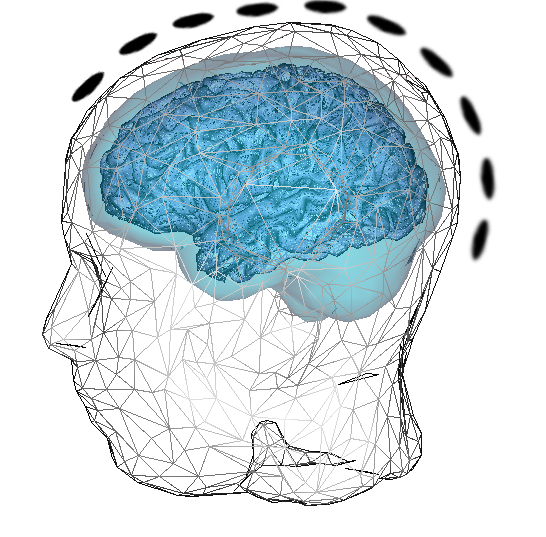
\includegraphics[height=9cm]{surf3.png}}

\noindent
Le problème direct consiste à estimer la valeur des potentiels et champs magnétiques qui seraient enregistrés \textbf{aux
capteurs} MEG/EEG étant donné une source d'activité.

\centerline{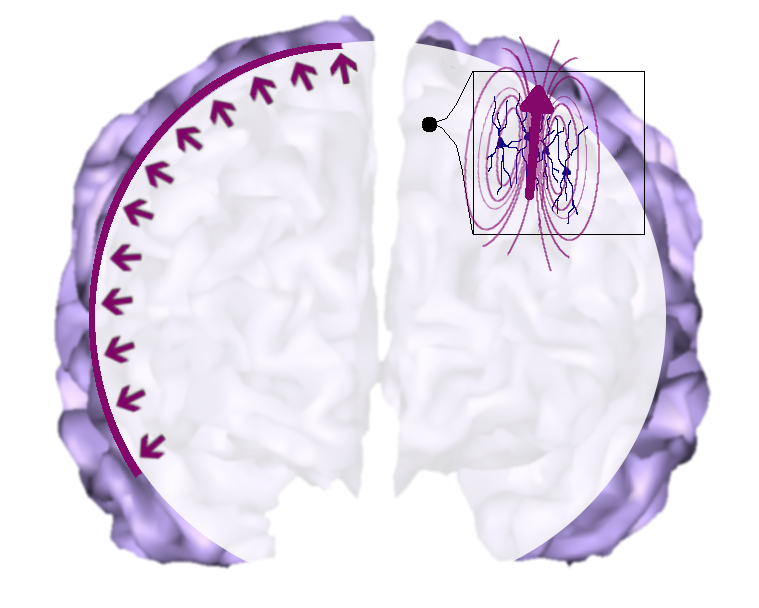
\includegraphics[height=10cm]{dipole.png}}

\noindent
\underline{Étape 1}~: on calcule le potentiel \textbf{sur toutes les surfaces } du modèle de tête (scalp, crâne extérieur et crâne intérieur pour un modèle à trois couches). Soit $\mathbf{X}$ un vecteur rassemblant  les valeurs du potentiel et des courants normaux sur les surfaces discrétisées. La méthode des éléments
frontières symétrique ramène à la résolution d'un système linéaire
suivant~:
\[
    \mathbf{HeadMat} . \mathbf{X} = \mathbf{SourceMat}
\]
Voir points \ref{sect: command assemble HeadMat}, \ref{sect: command assemble SourceMat} et \ref{sect: command invert HeadMat}.

\medskip

\noindent
\underline{Étape 2}~: les capteurs sont reliés au modèle de tête par plusieurs transformations linéaires représentées par des matrices. Ces matrices diffèrent entre la MEG et l'EEG. \\
\\
Pour l'EEG, le potentiel est interpolé aux positions des capteurs à partir des maillages de surfaces discrétisées, par une application linéaire~:\\
\[
    \left[ \mbox{valeur aux capteurs} \right] =
    \left[ \mbox{matrice de passage} \right] \times \left[ \mbox{valeurs sur le scalp} \right] \mbox{dans le cas de l'EEG.}
\]
Pour la MEG, l'équation de Biot et Savart montre qu'il y a deux contributions au champ magnétique: l'une provenant directement des sources d'activité électrique cérébrale, et l'autre provenant du courant ohmique, et calculable à partir du potentiel sur les surfaces du modèle.
Par conséquent, deux transformations linéaires doivent être calculées, l'une reliant les positions de sources aux capteurs MEG, et l'autre reliant les surfaces du modèle aux capteurs MEG.

Voir point \ref{sect: command assemble sensors}.

\medskip

\noindent
\underline{Étape 3}~: la matrice reliant les sources (à \textbf{position et orientation} fixée)  aux capteurs peut désormais être calculée. Cette matrice
est appelée matrice de gain et notée $\mathbf{G}$~ (point \ref{sect: command gain}). 
Appliquée à une matrice reflétant l'\textbf{activation} des sources, elle donne la solution du problème direct (point
\ref{sect: command direct}).
